\documentclass[11pt,a4paper]{article}
\usepackage[utf8]{inputenc}
\usepackage[T1]{fontenc}
\usepackage{lmodern}
\usepackage{microtype}
\usepackage[margin=2.5cm]{geometry}
\usepackage{amsmath,amssymb}
\usepackage[version=4]{mhchem}
\usepackage{siunitx}
\sisetup{per-mode=symbol, group-separator={\,}, group-minimum-digits=4}
\DeclareSIUnit\year{y}
\DeclareSIUnit\becquerel{Bq}
\usepackage{graphicx}
\usepackage{booktabs}
\usepackage{enumitem}
\usepackage[font=small,labelfont=bf]{caption}
\usepackage[most]{tcolorbox}
\usepackage{fancyhdr}
\usepackage[colorlinks=true,linkcolor=blue!60!black,citecolor=blue!60!black,urlcolor=blue!60!black]{hyperref}
\hypersetup{pdftitle={Introduction to Nuclear Physics: Radioactivity, Nuclear Energy and Computer Simulations}, pdfauthor={Zakaria Daoudi}}

\graphicspath{{figures/}}

% ---------- boxes ----------
\newtcolorbox{keybox}[1][]{colback=blue!4, colframe=blue!50!black, fonttitle=\bfseries,
  title=Key idea, #1}
\newtcolorbox{examplebox}[1][]{colback=green!4, colframe=green!40!black, fonttitle=\bfseries,
  title=Worked example, #1}
\newtcolorbox{codebox}[1][]{colback=orange!5, colframe=orange!70!black, fonttitle=\bfseries,
  title=Try it with the code, #1}
\newtcolorbox{furtherbox}[1][]{colback=gray!6, colframe=gray!60!black, fonttitle=\bfseries,
  title=Going further (first-year university), #1}

\newcommand{\nuc}[3]{\ensuremath{{}^{#1}_{#2}\mathrm{#3}}}   % \nuc{A}{Z}{X}
\newcommand{\iso}[2]{\ensuremath{{}^{#1}\mathrm{#2}}}         % \iso{A}{X}

\pagestyle{fancy}
\fancyhf{}
\fancyhead[L]{\small Introduction to Nuclear Physics}
\fancyhead[R]{\small Z. Daoudi}
\fancyfoot[C]{\thepage}
\setlength{\headheight}{14pt}

\title{\textbf{Introduction to Nuclear Physics}\\[4pt]
\large Radioactivity, nuclear energy and computer simulations}
\author{Zakaria Daoudi}
\date{}

\begin{document}
\maketitle
\thispagestyle{empty}

\begin{abstract}
\noindent These notes introduce the physics of the atomic nucleus: what nuclei are made of, why some of them are stable and others radioactive, how radioactive decay proceeds in time, and where nuclear energy comes from. They are written for students in the last years of high school and in the first year of university. The main text requires only algebra, exponentials and logarithms. Boxes marked \emph{Going further} use derivatives and simple differential equations, and can be skipped on a first reading. The notes come with a set of Python programs that simulate radioactive decay and compute nuclear energies from real data. The \emph{Try it with the code} boxes suggest experiments to do with them. All the numerical values of masses and half-lives are taken from the international evaluations AME2020~\cite{AME2020} and NUBASE2020~\cite{NUBASE2020}.
\end{abstract}

\setcounter{tocdepth}{1}
\tableofcontents
\newpage

%======================================================================
\section{The atomic nucleus}
%======================================================================

\subsection{A very small, very dense core}

Between 1909 and 1911, Hans Geiger and Ernest Marsden, working with Ernest Rutherford, sent alpha particles onto a thin gold foil. Most of them went straight through, but a few bounced back. In 1911, Rutherford concluded that almost all the mass of an atom is concentrated in a tiny, positively charged \emph{nucleus}, surrounded by light electrons.

The sizes involved are very different:
\begin{itemize}
  \item an atom has a radius of about $10^{-10}$~m;
  \item a nucleus has a radius of a few femtometres, $1~\text{fm} = 10^{-15}$~m.
\end{itemize}
The nucleus is therefore tens of thousands of times smaller than the atom. If the atom were the size of a football stadium, the nucleus would be a marble at its centre. Yet the nucleus carries more than $99.9\%$ of the mass of the atom.

\subsection{Protons and neutrons}

A nucleus is made of two kinds of particles, called \emph{nucleons}:
\begin{itemize}
  \item \textbf{protons}, with electric charge $+e$, where $e = \SI{1.602e-19}{C}$;
  \item \textbf{neutrons}, which have no electric charge.
\end{itemize}
Protons and neutrons have almost the same mass, about $1836$ times the mass of the electron (Table~\ref{tab:particles}).

A nucleus is described by two numbers:
\begin{itemize}
  \item the \textbf{atomic number} $Z$ is the number of protons. It fixes the chemical element: $Z=1$ is hydrogen, $Z=6$ carbon, $Z=92$ uranium;
  \item the \textbf{mass number} $A$ is the total number of nucleons. The number of neutrons is $N = A - Z$.
\end{itemize}
A nucleus with given $Z$ and $A$ is called a \emph{nuclide}. It is written $\nuc{A}{Z}{X}$, where X is the chemical symbol. For example, $\nuc{12}{6}{C}$ is carbon~12, with 6 protons and 6 neutrons, and $\nuc{238}{92}{U}$ is uranium~238, with 92 protons and 146 neutrons. Since the symbol already gives $Z$, we often simply write \iso{12}{C} or \iso{238}{U}.

Nuclides with the same $Z$ but different $A$ are \textbf{isotopes} of the same element. They have the same chemistry, since the chemistry is decided by the electrons, and hence by $Z$. But they can have very different nuclear properties. For example, \iso{12}{C} is stable, while \iso{14}{C} is radioactive.

\subsection{Units: electronvolts and atomic mass units}

The joule is a very large unit at the scale of a nucleus. Nuclear physicists use the \textbf{electronvolt} (eV), the energy gained by an electron accelerated through a potential difference of one volt:
\[
1~\text{eV} = \SI{1.602e-19}{J}, \qquad 1~\text{MeV} = 10^6~\text{eV} = \SI{1.602e-13}{J}.
\]
Chemical reactions involve energies of a few eV per atom. Nuclear reactions involve energies of a few MeV per nucleus, a million times more. This single fact explains why nuclear energy is so concentrated.

Masses are measured in \textbf{atomic mass units} (u), defined as one twelfth of the mass of a \iso{12}{C} atom:
\[
1~\text{u} = \SI{1.66054e-27}{kg}.
\]
By Einstein's relation $E = mc^2$, a mass can be expressed as an energy. The mass of 1~u corresponds to $931.494$~MeV, so we write $1~\text{u} = 931.494~\text{MeV}/c^2$.

\begin{table}[h]
\centering
\begin{tabular}{lccc}
\toprule
Particle & Charge & Mass (u) & Mass (MeV$/c^2$) \\
\midrule
Proton   & $+e$ & $1.007276$ & $938.272$ \\
Neutron  & $0$  & $1.008665$ & $939.565$ \\
Electron & $-e$ & $0.000549$ & $0.511$ \\
\bottomrule
\end{tabular}
\caption{The constituents of atoms~\cite{CODATA2018}. The neutron is heavier than the proton and the electron together, which is why a free neutron is radioactive (Section~\ref{sec:beta}).}
\label{tab:particles}
\end{table}

\subsection{Size and density of nuclei}

Experiments show that the radius of a nucleus grows with its mass number as
\begin{equation}
  R \approx r_0\, A^{1/3}, \qquad r_0 \approx 1.2~\text{fm}.
  \label{eq:radius}
\end{equation}
The volume $\frac{4}{3}\pi R^3 = \frac{4}{3}\pi r_0^3 A$ is therefore proportional to $A$: each nucleon occupies the same volume, as if nucleons were packed like marbles in a bag. All nuclei have the same density,
\[
\rho \approx \frac{A \times 1~\text{u}}{\frac{4}{3}\pi r_0^3 A}
= \frac{\SI{1.66e-27}{kg}}{\frac{4}{3}\pi\,(\SI{1.2e-15}{m})^3} \approx \SI{2.3e17}{kg/m^3}.
\]
A teaspoon of nuclear matter would weigh about a billion tonnes. This is the density inside neutron stars.

\subsection{What holds the nucleus together?}

Protons repel each other through the electric (Coulomb) force, and this repulsion is enormous at such small distances. Something else must hold the nucleus together: the \textbf{strong nuclear force}. Its main features are:
\begin{itemize}
  \item it is attractive and much stronger than the electric force at distances of about 1~fm;
  \item it has a very short range: it becomes negligible beyond 2 to 3~fm, so a nucleon only feels its nearest neighbours;
  \item it acts in the same way between protons and neutrons.
\end{itemize}
Neutrons therefore act as a ``glue'': they add strong attraction without adding electric repulsion.

%======================================================================
\section{Mass and binding energy}
%======================================================================

\subsection{The mass defect}

A remarkable fact is that a nucleus is \emph{lighter} than the sum of the masses of its protons and neutrons. Consider helium~4, with 2 protons and 2 neutrons. Using atomic masses, which include the electrons~\cite{AME2020}:
\begin{align*}
2\,m(\iso{1}{H}) + 2\,m_n &= 2 \times 1.007825 + 2 \times 1.008665 = 4.032980~\text{u},\\
m(\iso{4}{He}) &= 4.002603~\text{u}.
\end{align*}
The difference, $\Delta m = 0.030377$~u, is called the \textbf{mass defect}. It corresponds to the energy
\[
B = \Delta m\, c^2 = 0.030377 \times 931.494~\text{MeV} = 28.30~\text{MeV}.
\]
This is the \textbf{binding energy} of \iso{4}{He}: the energy one must supply to break the nucleus into its four nucleons. Conversely, it is the energy released when the nucleus is formed.

\begin{keybox}
The binding energy of a nucleus with $Z$ protons and $N$ neutrons is
\begin{equation}
  B = \left[ Z\, m(\iso{1}{H}) + N\, m_n - m(\text{atom}) \right] c^2 .
  \label{eq:binding}
\end{equation}
The larger $B/A$, the binding energy per nucleon, the more tightly bound the nucleus. Nuclear reactions release energy when they lead to more tightly bound nuclei.
\end{keybox}

Using the masses of hydrogen atoms instead of protons makes the electron masses cancel. The binding energy of the electrons themselves, at most about 1~MeV in total even for the heaviest atoms, is negligible here.

\subsection{The curve of binding energy}

Figure~\ref{fig:binding} shows $B/A$ for all the nuclei whose mass has been measured. The main features are:
\begin{itemize}
  \item $B/A$ is about $8$~MeV for most nuclei, so the total binding energy is roughly proportional to $A$;
  \item $B/A$ rises steeply for light nuclei. \iso{4}{He}, with $7.07$~MeV per nucleon, is unusually well bound;
  \item $B/A$ reaches a maximum of about $8.8$~MeV near iron and nickel. \iso{56}{Fe} has $8.790$~MeV, and the record holder is \iso{62}{Ni} with $8.795$~MeV;
  \item $B/A$ slowly decreases for heavy nuclei, down to $7.57$~MeV for \iso{238}{U}.
\end{itemize}

\begin{figure}[t]
\centering
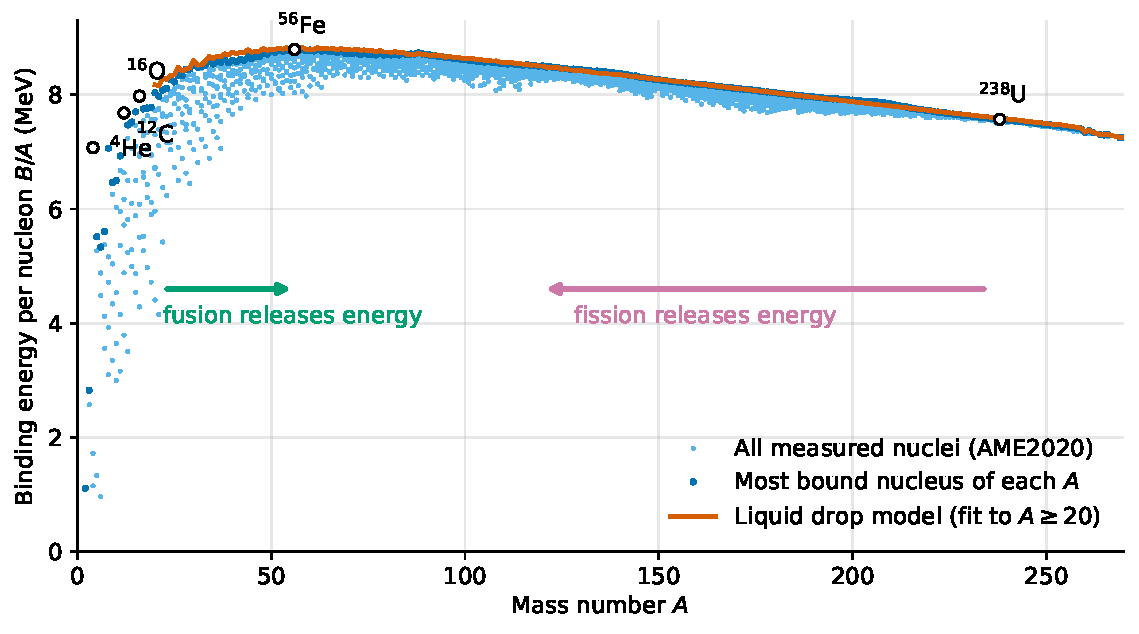
\includegraphics[width=\textwidth]{binding_energy}
\caption{Binding energy per nucleon of all nuclei with a measured mass (AME2020~\cite{AME2020}). Dark points are the most bound nucleus for each mass number $A$. The curve is the liquid drop model of Section~\ref{sec:liquid}, fitted to the data. Merging light nuclei (fusion) or splitting heavy ones (fission) moves towards the maximum and releases energy.}
\label{fig:binding}
\end{figure}

This curve is the key to nuclear energy. Moving from either end towards the maximum releases energy:
\begin{itemize}
  \item joining two light nuclei into a heavier one is \textbf{fusion}; it powers the stars;
  \item splitting a heavy nucleus into two medium ones is \textbf{fission}; it powers nuclear reactors.
\end{itemize}

\begin{examplebox}
\textbf{Why does fission release about 200 MeV?} A uranium nucleus ($A \approx 236$ after absorbing a neutron) has $B/A \approx 7.6$~MeV. It splits into two fragments of $A \approx 118$, for which $B/A \approx 8.5$~MeV. The total binding energy increases by about
\[
236 \times (8.5 - 7.6)~\text{MeV} \approx 210~\text{MeV}.
\]
This energy is released, mostly as kinetic energy of the fragments. Compare this with the burning of one carbon atom, which releases about 4~eV: the fission of one nucleus releases about 50 million times more energy.
\end{examplebox}

\subsection{The liquid drop model}
\label{sec:liquid}

Because the strong force has a short range and all nuclei have the same density, a nucleus behaves somewhat like a drop of liquid. This picture leads to the \textbf{semi-empirical mass formula} of Bethe and von Weizsäcker, which gives the binding energy as a sum of five terms:
\begin{equation}
  B(Z,A) = a_V A \;-\; a_S A^{2/3} \;-\; a_C \frac{Z(Z-1)}{A^{1/3}} \;-\; a_A \frac{(N-Z)^2}{A} \;+\; \delta(Z,A).
  \label{eq:semf}
\end{equation}
Each term has a simple meaning:
\begin{description}[leftmargin=1em]
  \item[Volume term $a_V A$.] Each nucleon is bound to its neighbours, so the binding grows like the number of nucleons.
  \item[Surface term $-a_S A^{2/3}$.] Nucleons at the surface have fewer neighbours and are less bound. The surface area grows like $R^2 \propto A^{2/3}$.
  \item[Coulomb term $-a_C Z(Z-1)/A^{1/3}$.] Each of the $Z(Z-1)/2$ pairs of protons repels, with an energy that decreases with the distance, $\propto 1/R \propto A^{-1/3}$.
  \item[Asymmetry term $-a_A (N-Z)^2/A$.] A quantum effect (the Pauli principle): nuclei prefer equal numbers of protons and neutrons.
  \item[Pairing term $\delta$.] Nucleons like to form pairs: $\delta = +a_P/\sqrt{A}$ when $Z$ and $N$ are both even, $-a_P/\sqrt{A}$ when both are odd, and $0$ when $A$ is odd.
\end{description}
The five coefficients are found by fitting the formula to the measured binding energies. The program \texttt{nuclear\_energy.py} does exactly this with the 2455 measured nuclei with $A \geq 20$ in AME2020, and finds
\[
a_V = 15.46, \quad a_S = 17.02, \quad a_C = 0.699, \quad a_A = 22.62, \quad a_P = 12.17 \quad (\text{in MeV}).
\]
With only five parameters, the formula reproduces binding energies of up to 2000~MeV with a typical error of 3~MeV, as Figure~\ref{fig:binding} shows. Its remaining deviations, in particular for some ``magic'' numbers of protons or neutrons (2, 8, 20, 28, 50, 82, 126) that are especially stable, are explained by the \emph{shell model} of the nucleus, which is beyond these notes.

\begin{codebox}
Run \texttt{python3 nuclear\_energy.py}. The program prints the binding energies of a few nuclei, fits the five coefficients of Eq.~\eqref{eq:semf} and plots the curve of Figure~\ref{fig:binding}. You can compute the binding energy of any nucleus in a Python session:
\begin{verbatim}
from nuclear_energy import binding_energy
print(binding_energy("208Pb") / 208)    # MeV per nucleon
\end{verbatim}
\end{codebox}

\subsection{Stable and unstable nuclei}

Of the more than 3000 nuclides observed so far, only about 250 are stable. Figure~\ref{fig:chart} places the nuclides of the NUBASE2020 evaluation on a map, the \textbf{chart of nuclides}, with $N$ horizontally and $Z$ vertically. The stable nuclei form a narrow \emph{valley of stability}:
\begin{itemize}
  \item for light nuclei, the stable ones have $N \approx Z$ (for example \iso{4}{He}, \iso{12}{C}, \iso{16}{O});
  \item for heavy nuclei, they have more neutrons than protons (\iso{208}{Pb} has 82 protons and 126 neutrons). The extra neutrons dilute the electric repulsion between the protons, which grows like $Z^2$;
  \item no nucleus heavier than lead ($Z = 82$) is stable. Bismuth~209 comes close: its half-life, $2 \times 10^{19}$~years, is a billion times the age of the Universe.
\end{itemize}
Nuclei away from the valley are radioactive. They move towards it by emitting particles, as we will now see.

\begin{figure}[t]
\centering
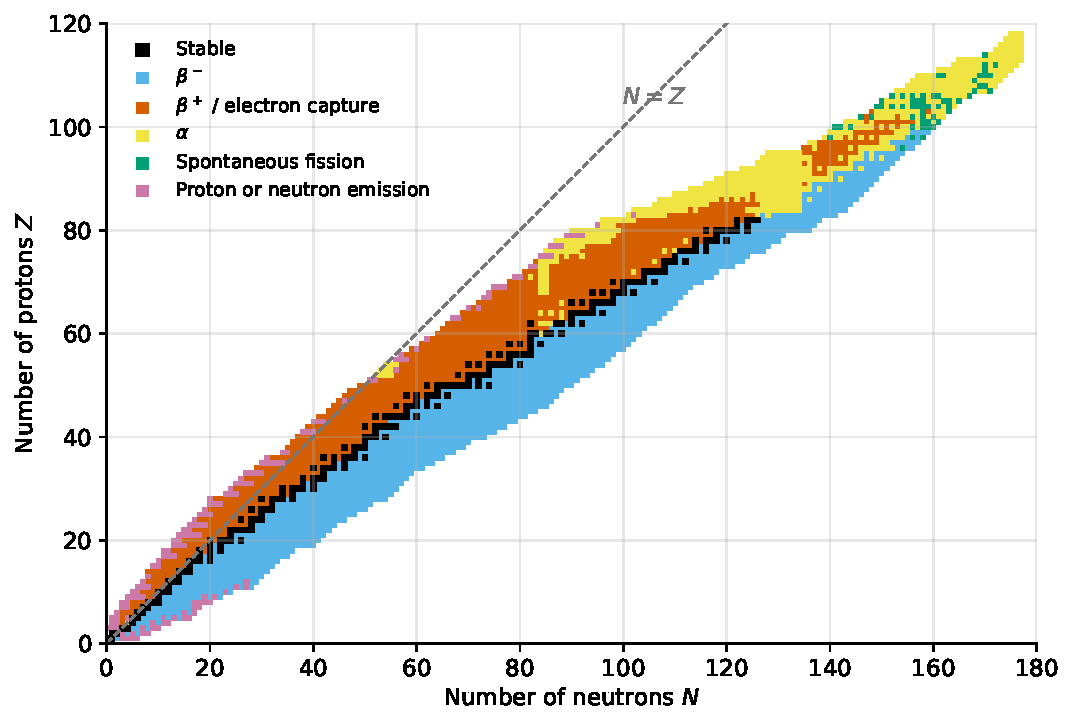
\includegraphics[width=0.85\textwidth]{chart}
\caption{Chart of nuclides: all ground states in NUBASE2020, coloured by their main decay mode (NUBASE2020~\cite{NUBASE2020}). Black squares are stable nuclei. Nuclei with too many neutrons (below the valley) undergo $\beta^-$ decay, those with too many protons undergo $\beta^+$ decay or electron capture, and the heaviest ones undergo $\alpha$ decay or spontaneous fission.}
\label{fig:chart}
\end{figure}

\begin{furtherbox}
The liquid drop formula predicts where the valley lies. For fixed $A$, the most stable $Z$ maximizes $B(Z,A)$. Setting $\partial B/\partial Z = 0$ and neglecting the small pairing term and the difference between $Z(Z-1)$ and $Z^2$ gives
\[
Z_{\text{stable}} \approx \frac{A}{2 + (a_C/2a_A)\,A^{2/3}} = \frac{A}{2 + 0.0154\,A^{2/3}}.
\]
For $A = 238$, this gives $Z \approx 91.8$, close to uranium ($Z=92$). For light nuclei the Coulomb term is negligible and $Z \approx A/2$, that is $N \approx Z$.
\end{furtherbox}

%======================================================================
\section{Radioactivity}
%======================================================================

\subsection{A short history}

In 1896, Henri Becquerel discovered that uranium salts emit a penetrating radiation, even in the dark. Marie and Pierre Curie showed that this property, which they called \emph{radioactivity}, belongs to the atoms themselves, and discovered two new radioactive elements, polonium and radium. Rutherford then distinguished two types of radiation by their penetrating power, which he named $\alpha$ and $\beta$. A third, much more penetrating type, discovered by Paul Villard in 1900, was later named $\gamma$. The three types also behave differently in a magnetic field, which deflects $\alpha$ and $\beta$ in opposite directions and does not deflect $\gamma$.

\subsection{Conservation laws}

In every nuclear decay or reaction, the following quantities are conserved:
\begin{itemize}
  \item the \textbf{electric charge}: the sum of the $Z$ values (counting $-1$ for an electron and $+1$ for a positron);
  \item the \textbf{number of nucleons}: the sum of the $A$ values;
  \item the \textbf{energy}, including the mass energy $mc^2$, and the \textbf{momentum}.
\end{itemize}
The first two rules, the \emph{displacement laws} of Soddy and Fajans, are enough to identify the nucleus produced by a decay.

A decay is only possible if it releases energy, that is, if the total mass decreases. The energy released is the \textbf{$Q$-value}:
\begin{equation}
  Q = \left( m_{\text{initial}} - m_{\text{final}} \right) c^2 > 0 .
  \label{eq:Q}
\end{equation}
It is shared as kinetic energy among the products.

\subsection{Alpha decay}

An $\alpha$ particle is a helium~4 nucleus, \nuc{4}{2}{He}: two protons and two neutrons. Heavy nuclei can lower their energy by emitting one:
\[
\nuc{A}{Z}{X} \;\longrightarrow\; \nuc{A-4}{Z-2}{Y} + \nuc{4}{2}{He}.
\]
For example, the decay of uranium~238 is
\[
\ce{^{238}_{92}U -> ^{234}_{90}Th + ^{4}_{2}He}, \qquad Q = 4.27~\text{MeV}.
\]
Because \iso{4}{He} is so tightly bound, emitting it as a whole is much more favourable than emitting separate nucleons. By momentum conservation, the light $\alpha$ particle carries most of the energy: its kinetic energy is $Q \times (A-4)/A = 4.20$~MeV, and the thorium nucleus recoils with the remaining $0.07$~MeV. For a given transition, all the $\alpha$ particles therefore have the same energy. (Some decays lead to an excited state of the daughter, which gives a second, slightly lower $\alpha$ energy.)

Alpha particles are stopped by a sheet of paper or a few centimetres of air, but they are very harmful if the radioactive substance is inhaled or swallowed.

\begin{furtherbox}
The $\alpha$ particle is held inside the nucleus by a barrier created by the Coulomb repulsion. For \iso{238}{U}, this barrier is about 30~MeV high, much more than the 4.27~MeV available. Classically the $\alpha$ particle could never escape. Quantum mechanics allows it to \emph{tunnel} through the barrier with a small probability at each attempt. The tunnelling probability depends extremely strongly on the energy, which explains why the half-lives of $\alpha$ emitters range from less than a microsecond to billions of years for $\alpha$ energies between about 9 and 4~MeV (the Geiger--Nuttall law). This explanation, given by George Gamow in 1928, was one of the first triumphs of quantum mechanics.
\end{furtherbox}

\subsection{Beta decay}
\label{sec:beta}

In $\beta$ decay, a neutron turns into a proton inside the nucleus, or the reverse. The number of nucleons $A$ does not change. This transformation is caused by the \emph{weak} interaction.

\paragraph{Beta-minus decay.} A nucleus with too many neutrons turns a neutron into a proton, emitting an electron and an antineutrino:
\[
n \longrightarrow p + e^- + \bar{\nu}_e ,
\qquad
\nuc{A}{Z}{X} \longrightarrow \nuc{A}{Z+1}{Y} + e^- + \bar{\nu}_e .
\]
Example: \ce{^{14}_{6}C -> ^{14}_{7}N + e- + $\bar{\nu}_e$}, with $Q = 0.156$~MeV. A free neutron is itself radioactive, with a half-life of about 10 minutes, because it is heavier than a proton and an electron together.

\paragraph{Beta-plus decay.} A nucleus with too many protons turns a proton into a neutron, emitting a positron (the antiparticle of the electron) and a neutrino:
\[
\nuc{A}{Z}{X} \longrightarrow \nuc{A}{Z-1}{Y} + e^+ + \nu_e .
\]
Example: \ce{^{22}_{11}Na -> ^{22}_{10}Ne + e+ + $\nu_e$}. The positron quickly meets an electron and both annihilate into two $\gamma$ photons of $0.511$~MeV each. This is the principle of the PET scan in medicine.

\paragraph{Electron capture.} Instead of emitting a positron, the nucleus can capture one of its own atomic electrons: $p + e^- \to n + \nu_e$. It competes with $\beta^+$ decay. For example, potassium~40 decays by $\beta^-$ in $89.3\%$ of cases and by $\beta^+$ or electron capture in $10.7\%$~\cite{NUBASE2020}.

\paragraph{The neutrino.} In $\beta$ decay, the electron does not always have the same energy: its energies form a continuous spectrum, from zero up to $Q$. In 1930, to save energy conservation, Wolfgang Pauli proposed that an invisible, neutral and very light particle carries away the missing energy. This \emph{neutrino} interacts so weakly with matter that it was only detected in 1956, near a nuclear reactor.

Beta particles are stopped by a few millimetres of aluminium.

\subsection{Gamma emission}

After an $\alpha$ or $\beta$ decay, the daughter nucleus is often left in an \emph{excited state}. Just like an atom, it returns to its ground state by emitting a photon. Because nuclear energies are thousands to millions of times larger than atomic energies, these photons are \textbf{gamma rays}, with energies from tens of keV to a few MeV:
\[
\nuc{A}{Z}{X}^* \longrightarrow \nuc{A}{Z}{X} + \gamma .
\]
Neither $Z$ nor $A$ changes. Gamma rays are very penetrating: absorbing most of them requires several centimetres of lead or about a metre of concrete. Some excited states live long enough to be used on their own. Technetium~99m (``m'' for metastable), with a half-life of 6.0~hours, is the most used radioactive tracer in medical imaging.

\subsection{Energy of a decay from atomic masses}

Mass tables give the masses of neutral \emph{atoms}. With atomic masses, the electrons automatically balance in $\alpha$ decay, $\beta^-$ decay and electron capture, so that Eq.~\eqref{eq:Q} can be used directly. In $\beta^+$ decay, the daughter atom has one electron too many and a positron is created, so the energy available is smaller by $2 m_e c^2 = 1.022$~MeV:
\[
Q_{\beta^+} = \left[ m(\text{parent atom}) - m(\text{daughter atom}) - 2 m_e \right] c^2 .
\]
Table~\ref{tab:Q} gives the $Q$-values of several decays and reactions, computed by the program from the AME2020 masses.

\begin{table}[t]
\centering
\begin{tabular}{llr}
\toprule
Process & Equation & $Q$ (MeV) \\
\midrule
$\alpha$ decay & \ce{^{238}U -> ^{234}Th + ^{4}He} & $4.270$ \\
$\alpha$ decay & \ce{^{210}Po -> ^{206}Pb + ^{4}He} & $5.408$ \\
$\beta^-$ decay & \ce{^{14}C -> ^{14}N + e- + $\bar{\nu}$} & $0.156$ \\
$\beta^-$ decay & \ce{^{3}H -> ^{3}He + e- + $\bar{\nu}$} & $0.0186$ \\
$\beta^+$ decay & \ce{^{22}Na -> ^{22}Ne + e+ + $\nu$} & $1.821$ \\
Fission & \ce{^{235}U + n -> ^{141}Ba + ^{92}Kr + 3n} & $173.3$ \\
Fusion & \ce{^{2}H + ^{3}H -> ^{4}He + n} & $17.59$ \\
Fusion & \ce{^{2}H + ^{2}H -> ^{3}He + n} & $3.27$ \\
Proton--proton chain & \ce{4 ^{1}H -> ^{4}He + 2 e+ + 2 $\nu$} & $26.73$ \\
\bottomrule
\end{tabular}
\caption{Energy released by some decays and reactions, computed with \texttt{nuclear\_energy.py} from the AME2020 atomic masses~\cite{AME2020}. For the proton--proton chain, the value includes the annihilation of the two positrons with two electrons.}
\label{tab:Q}
\end{table}

\begin{examplebox}
\textbf{The $\alpha$ decay of \iso{238}{U}.} The atomic masses are $m(\iso{238}{U}) = 238.050787$~u, $m(\iso{234}{Th}) = 234.043600$~u and $m(\iso{4}{He}) = 4.002603$~u. Then
\begin{align*}
\Delta m &= 238.050787 - 234.043600 - 4.002603 = 0.004584~\text{u},\\
Q &= 0.004584 \times 931.494~\text{MeV} = 4.27~\text{MeV}.
\end{align*}
\end{examplebox}

%======================================================================
\section{The law of radioactive decay}
%======================================================================

\subsection{A random process}

Radioactive decay is \emph{random}. It is impossible to predict when a given nucleus will decay. A nucleus does not age: a uranium nucleus that has existed for 4 billion years has exactly the same chance to decay in the next second as a newly formed one. The only thing we know is the probability of decay per unit time, called the \textbf{decay constant} $\lambda$, which is characteristic of each nuclide. During a short time $\Delta t$, each nucleus has a probability $\lambda\,\Delta t$ of decaying.

If we have $N$ nuclei, the average number that decay during $\Delta t$ is therefore
\begin{equation}
  \Delta N = -\lambda N \,\Delta t .
  \label{eq:dN}
\end{equation}
The number of decays is proportional to the number of nuclei present: the more nuclei, the more decays.

\subsection{Exponential decay and half-life}

The solution of Eq.~\eqref{eq:dN} is the \textbf{law of radioactive decay}:
\begin{keybox}
\begin{equation}
  N(t) = N_0\, e^{-\lambda t},
  \label{eq:decay}
\end{equation}
where $N_0$ is the number of nuclei at time $t=0$. The \textbf{half-life} $T_{1/2}$ is the time after which half of the nuclei have decayed:
\begin{equation}
  T_{1/2} = \frac{\ln 2}{\lambda} \approx \frac{0.693}{\lambda},
  \qquad
  N(t) = N_0 \left( \frac{1}{2} \right)^{t/T_{1/2}} .
  \label{eq:halflife}
\end{equation}
\end{keybox}

After one half-life, $N_0/2$ nuclei remain; after two, $N_0/4$; after three, $N_0/8$; and so on (Figure~\ref{fig:decaylaw}). The half-life does not depend on how many nuclei there are, nor on the temperature, the pressure or the chemical state. Half-lives range from less than $10^{-20}$~s to more than $10^{24}$~years. Table~\ref{tab:halflives} gives some examples.

\begin{figure}[!hb]
\centering
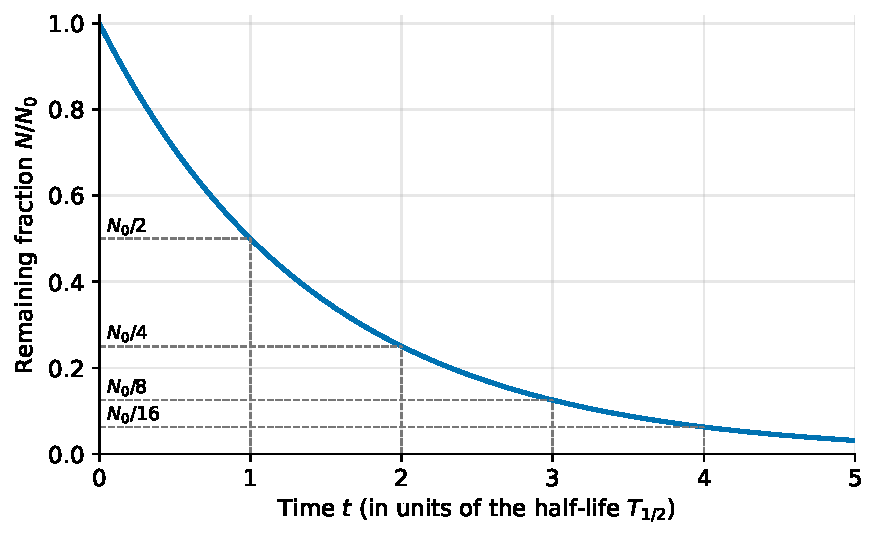
\includegraphics[width=0.7\textwidth]{decay_law}
\caption{Exponential decay: the number of nuclei is halved after each half-life.}
\label{fig:decaylaw}
\end{figure}

\begin{table}[!hb]
\centering
\begin{tabular}{llll}
\toprule
Nuclide & Decay & Half-life & Where you meet it \\
\midrule
\iso{15}{O} & $\beta^+$ & $122$~s & PET scans of blood flow \\
\iso{18}{F} & $\beta^+$ & $109.7$~min & PET scans \\
\iso{99m}{Tc} & $\gamma$ & $6.01$~h & Medical imaging \\
\iso{222}{Rn} & $\alpha$ & $3.82$~days & Natural radon gas in houses \\
\iso{131}{I} & $\beta^-$ & $8.02$~days & Thyroid treatment, reactor accidents \\
\iso{60}{Co} & $\beta^-$ & $5.27$~years & Radiotherapy, sterilization \\
\iso{3}{H} (tritium) & $\beta^-$ & $12.32$~years & Fusion fuel, luminous watches \\
\iso{137}{Cs} & $\beta^-$ & $30.04$~years & Nuclear waste, fallout \\
\iso{241}{Am} & $\alpha$ & $432.6$~years & Smoke detectors \\
\iso{226}{Ra} & $\alpha$ & $1600$~years & Discovered by the Curies \\
\iso{14}{C} & $\beta^-$ & $5700$~years & Radiocarbon dating \\
\iso{235}{U} & $\alpha$ & $7.04 \times 10^8$~years & Nuclear fuel \\
\iso{40}{K} & $\beta^-$, $\beta^+$/EC & $1.248 \times 10^9$~years & Present in our body \\
\iso{238}{U} & $\alpha$ & $4.463 \times 10^9$~years & Natural uranium \\
\bottomrule
\end{tabular}
\caption{Half-lives of some radioactive nuclides (NUBASE2020~\cite{NUBASE2020}).}
\label{tab:halflives}
\end{table}

\begin{furtherbox}
When $\Delta t \to 0$, Eq.~\eqref{eq:dN} becomes the differential equation
\[
\frac{dN}{dt} = -\lambda N .
\]
Separating the variables, $dN/N = -\lambda\,dt$, and integrating from $0$ to $t$ gives $\ln(N/N_0) = -\lambda t$, which is Eq.~\eqref{eq:decay}. Setting $N = N_0/2$ gives $e^{-\lambda T_{1/2}} = 1/2$, so $T_{1/2} = \ln 2/\lambda$.

The \textbf{mean lifetime} of a nucleus is the average time it lives before decaying:
\[
\tau = \frac{1}{N_0}\int_0^\infty t \left| \frac{dN}{dt} \right| dt = \int_0^\infty \lambda t\, e^{-\lambda t}\,dt = \frac{1}{\lambda} = \frac{T_{1/2}}{\ln 2} \approx 1.44\, T_{1/2}.
\]
\end{furtherbox}

\subsection{Activity}

What a Geiger counter measures is not the number of nuclei but the number of decays per second, called the \textbf{activity}:
\begin{equation}
  A(t) = \lambda N(t) = A_0\, e^{-\lambda t}.
  \label{eq:activity}
\end{equation}
The activity decreases with the same half-life as the number of nuclei. Its unit is the \textbf{becquerel}: $1~\text{Bq} = 1$ decay per second. An older unit is the curie, $1~\text{Ci} = \SI{3.7e10}{Bq}$, originally defined as the activity of one gram of radium.

\begin{examplebox}
\textbf{Activity of one gram of radium~226.} The number of atoms is
\[
N = \frac{1~\text{g}}{226~\text{g/mol}} \times \SI{6.022e23}{mol^{-1}} = \num{2.66e21}.
\]
The half-life is $1600$~years $= 1600 \times \SI{3.156e7}{s} = \SI{5.05e10}{s}$, so $\lambda = 0.693/\SI{5.05e10}{s} = \SI{1.37e-11}{s^{-1}}$, and
\[
A = \lambda N = \SI{3.66e10}{Bq} \approx 1~\text{Ci}.
\]
\end{examplebox}

\begin{examplebox}
\textbf{We are radioactive.} A human body of 70~kg contains about 140~g of potassium, of which $0.0117\%$ is radioactive \iso{40}{K}~\cite{NUBASE2020}. This makes
\[
N = \frac{140}{39.1} \times \num{6.022e23} \times \num{1.17e-4} = \num{2.5e20}
\]
nuclei of \iso{40}{K}. With $T_{1/2} = \num{1.248e9}$~years $= \SI{3.94e16}{s}$, the activity is $A = (0.693/\SI{3.94e16}{s}) \times \num{2.5e20} \approx 4400$~Bq. About 4400 potassium nuclei decay in your body every second.
\end{examplebox}

\subsection{Randomness and fluctuations}

The exponential law~\eqref{eq:decay} describes the \emph{average} behaviour. With a small number of nuclei, the actual number fluctuates around it. Since each nucleus decays independently, the number that survive until time $t$ follows a binomial distribution, with mean $N_0 e^{-\lambda t}$ and standard deviation
\[
\sigma = \sqrt{N_0\, e^{-\lambda t}\left(1 - e^{-\lambda t}\right)} .
\]
The relative fluctuation $\sigma/N$ decreases like $1/\sqrt{N_0}$: with 100 nuclei the fluctuations are clearly visible, while with $10^{20}$ nuclei, as in any macroscopic sample, they are completely negligible (Figure~\ref{fig:mc}).

\begin{figure}[t]
\centering
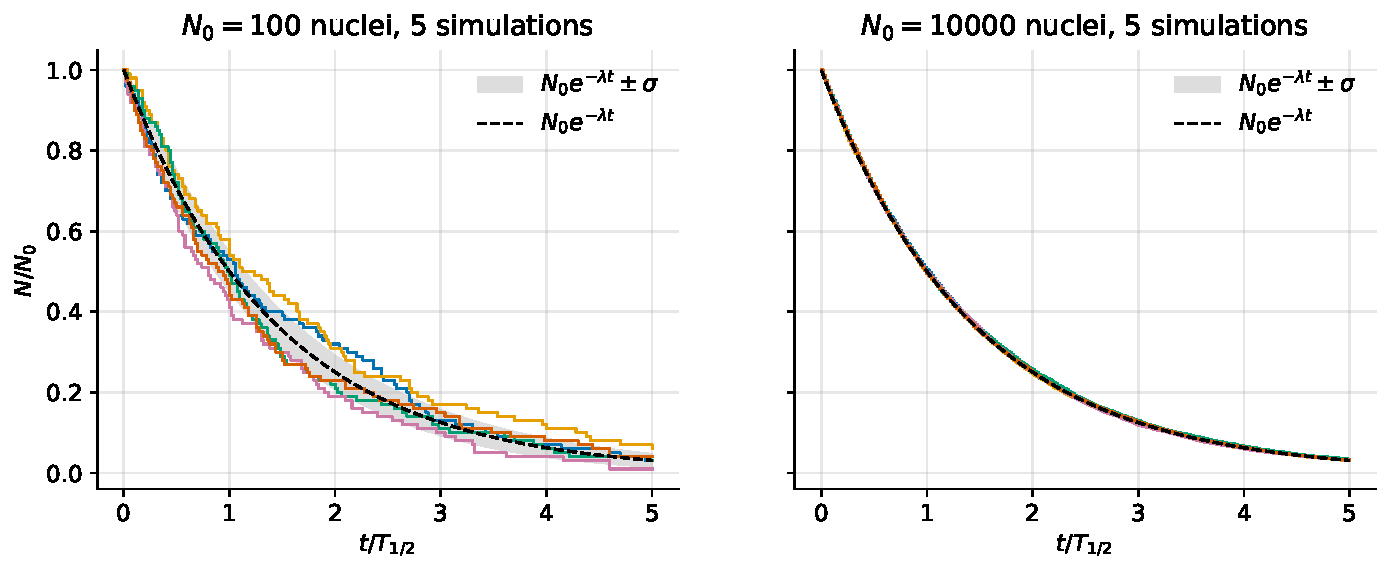
\includegraphics[width=\textwidth]{monte_carlo}
\caption{Monte Carlo simulations of radioactive decay. Each coloured line is one simulation in which every nucleus decays at random. The grey band shows the exponential law $\pm$ one standard deviation. With 100 nuclei (left) the random fluctuations are large; with $10^4$ nuclei (right) they are barely visible.}
\label{fig:mc}
\end{figure}

\begin{codebox}
Run \texttt{python3 nuclear.py} and choose simulation 4, \emph{Monte Carlo decay}. The program follows each nucleus: during each time step $\Delta t$, every remaining nucleus decays with probability $p = 1 - e^{-\lambda \Delta t}$. Try $N_0 = 10$, $100$ and $\num{10000}$ with 5 simulations each. How long does it take for the last nucleus to decay? Is it always the same?
\end{codebox}

\subsection{Solving the decay law with a computer: Euler's method}

The decay law can be solved step by step, which is how a computer solves equations that have no exact solution. Starting from $N_0$, we apply Eq.~\eqref{eq:dN} repeatedly with a small time step $\Delta t$:
\[
N_{i+1} = N_i - \lambda N_i\, \Delta t, \qquad t_{i+1} = t_i + \Delta t .
\]
This is \textbf{Euler's method}. It is exact only in the limit $\Delta t \to 0$. Figure~\ref{fig:euler} compares it with the exact solution: with only 8 steps for 5 half-lives, the result is poor; with 100 steps it is already very close. The error at a given time is proportional to the step size: halving $\Delta t$ halves the error. Euler's method is said to be of \emph{first order}.

\begin{figure}[t]
\centering
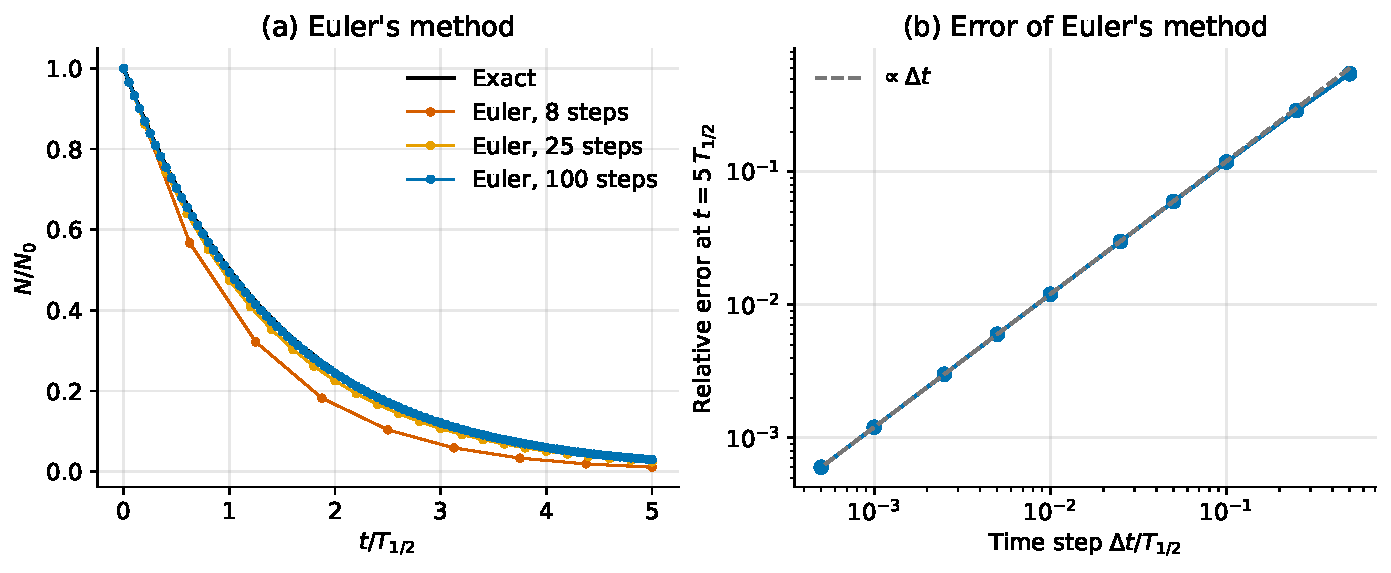
\includegraphics[width=\textwidth]{euler}
\caption{(a) Euler's method compared with the exact solution $N_0 e^{-\lambda t}$. (b) The relative error at $t = 5\,T_{1/2}$ is proportional to the time step $\Delta t$.}
\label{fig:euler}
\end{figure}

\begin{codebox}
Run \texttt{python3 radioactivity.py}, choose a nuclide and compare Euler's method with the exact solution for 10, 100 and \num{100000} steps. The program prints the final number of nuclei obtained both ways. Program \texttt{nuclear.py}, simulation 1, also shows the activity.
\end{codebox}

\begin{furtherbox}
Euler's method can even become \emph{unstable}. Since $N_{i+1} = (1 - \lambda \Delta t)\,N_i$, the numbers oscillate in sign if $\lambda \Delta t > 1$, and blow up if $\lambda \Delta t > 2$. This is a real danger for decay chains, where parent and daughter can have very different half-lives (Section~\ref{sec:chains}). For \iso{238}{U} $\to$ \iso{234}{Th}, a time step adapted to uranium (millions of years) is tens of millions of times larger than the half-life of thorium (24 days). For this reason, the programs use the exact solutions for decay chains.
\end{furtherbox}

%======================================================================
\section{Decay chains}
\label{sec:chains}
%======================================================================

\subsection{Parent and daughter}

The daughter of a radioactive decay is often radioactive itself. In the simplest chain, a parent P decays into a daughter D, which decays into a stable nucleus:
\[
\text{P} \xrightarrow{\;\lambda_P\;} \text{D} \xrightarrow{\;\lambda_D\;} \text{stable}.
\]
The parent follows the usual law, $N_P(t) = N_0 e^{-\lambda_P t}$. The daughter is produced by the decays of the parent and destroyed by its own decays:
\begin{equation}
  \Delta N_D = \left( \lambda_P N_P - \lambda_D N_D \right) \Delta t .
  \label{eq:chain}
\end{equation}
If there are no daughter nuclei at $t = 0$, the solution is
\begin{equation}
  N_D(t) = N_0\, \frac{\lambda_P}{\lambda_D - \lambda_P} \left( e^{-\lambda_P t} - e^{-\lambda_D t} \right).
  \label{eq:bateman}
\end{equation}
Harry Bateman gave the general solution for chains of any length in 1910~\cite{Bateman1910}.

\begin{furtherbox}
Check that Eq.~\eqref{eq:bateman} solves $dN_D/dt = \lambda_P N_P - \lambda_D N_D$ with $N_D(0) = 0$. When $\lambda_D = \lambda_P = \lambda$, the formula has the form $0/0$. Taking the limit gives $N_D(t) = N_0\, \lambda t\, e^{-\lambda t}$.
\end{furtherbox}

\subsection{Radioactive equilibrium}

The behaviour of the chain depends on which of the two nuclides lives longer (Figure~\ref{fig:chains}).

\paragraph{Secular equilibrium ($T_P \gg T_D$).} When the parent lives much longer than the daughter, the daughter accumulates until it decays as fast as it is produced. After a few daughter half-lives, $e^{-\lambda_D t}$ becomes negligible and
\[
\lambda_D N_D = \lambda_P N_P, \qquad\text{that is,}\qquad A_D = A_P .
\]
The two activities are equal. Figure~\ref{fig:chains}(a) shows this for thorium~232 ($1.40 \times 10^{10}$~years) and its daughter radium~228 ($5.75$~years). In a uranium ore that has not been disturbed for millions of years, all the members of the uranium decay series have the same activity.

\paragraph{Transient equilibrium ($T_P > T_D$).} When the parent lives longer than the daughter, but not by much, the daughter activity first grows, overtakes the parent activity and then decreases with the half-life of the \emph{parent}. The ratio of activities becomes constant:
\[
\frac{A_D}{A_P} = \frac{\lambda_D}{\lambda_D - \lambda_P} = \frac{T_P}{T_P - T_D} .
\]
Figure~\ref{fig:chains}(b) shows barium~140 ($12.75$~days) and lanthanum~140 ($40.3$~hours), for which $A_D/A_P \to 1.15$. The same principle is used in hospitals: technetium~99m is ``milked'' from a generator containing its parent, molybdenum~99 (66~hours).

\paragraph{No equilibrium ($T_P < T_D$).} If the daughter lives longer than the parent, the parent disappears first and the daughter then decays with its own half-life.

\begin{figure}[t]
\centering
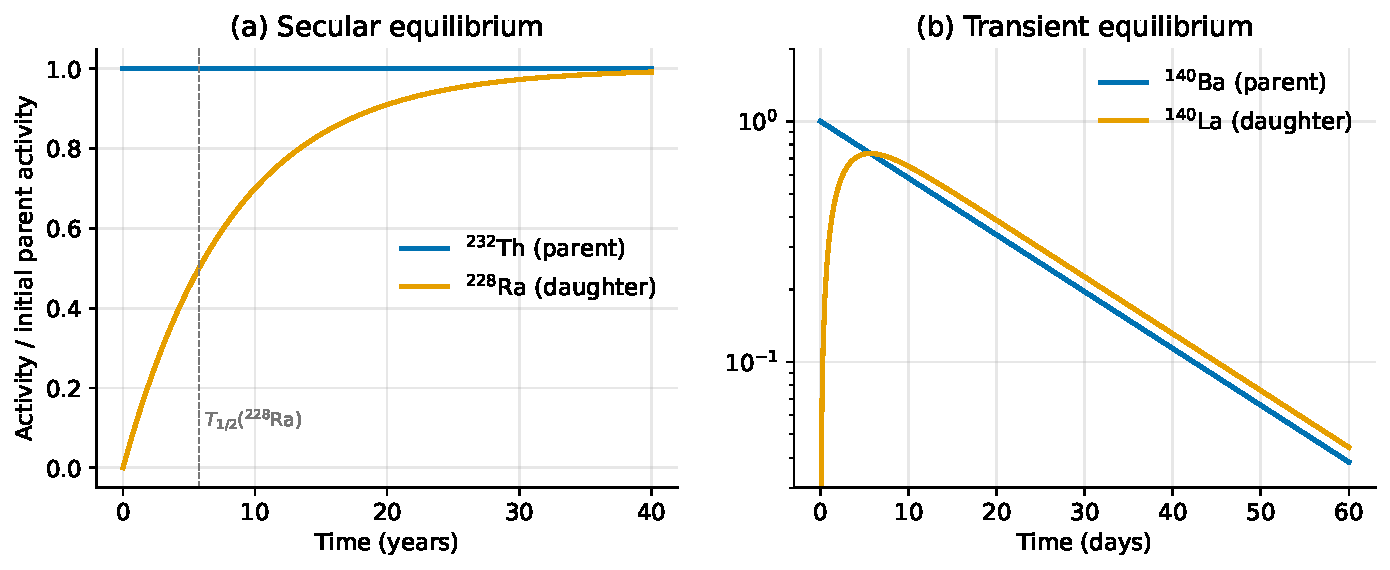
\includegraphics[width=\textwidth]{chains}
\caption{Activities in two decay chains, computed with the exact solution~\eqref{eq:bateman}. (a) Secular equilibrium: the activity of \iso{228}{Ra} grows until it equals that of its very long-lived parent \iso{232}{Th}. (b) Transient equilibrium: the activity of \iso{140}{La} overtakes that of its parent \iso{140}{Ba}, then both decay with the parent's half-life.}
\label{fig:chains}
\end{figure}

\subsection{Natural decay series and branching}

Uranium~238 does not become stable in one step. It goes through a chain of 14 decays, 8 $\alpha$ and 6 $\beta^-$, which ends with stable lead~206. The number of $\alpha$ decays follows from the mass numbers: each $\alpha$ decay reduces $A$ by 4 and $238 - 206 = 32 = 8 \times 4$. The $\alpha$ decays reduce $Z$ by 16, from 92 to 76, and 6 $\beta^-$ decays bring it back to 82. Radon~222, a gas produced in this series, seeps out of the ground and is the main source of natural radiation exposure in many regions.

Some nuclides can decay in two different ways; this is called \textbf{branching}. For example, bismuth~212 decays by $\beta^-$ in $64\%$ of cases and by $\alpha$ in $36\%$~\cite{NUBASE2020}. Each daughter then receives the corresponding fraction, the \emph{branching ratio}, of the parent decays.

\begin{codebox}
In \texttt{python3 nuclear.py}, simulation 2 follows a parent--daughter chain. The program suggests the daughters of \iso{238}{U}, \iso{235}{U} and \iso{232}{Th}, and you can enter any other half-life. Choose \iso{232}{Th} and a total time of 50 years to see the secular equilibrium building up. Simulation 3 adds a branching into two daughters.
\end{codebox}

%======================================================================
\section{Applications of radioactivity}
%======================================================================

\subsection{Radiocarbon dating}

Carbon~14 is continuously produced in the upper atmosphere, when neutrons from cosmic rays hit nitrogen: \ce{^{14}N + n -> ^{14}C + p}. It mixes with ordinary carbon in the carbon dioxide of the air, and is absorbed by plants and animals. As long as an organism is alive, the proportion of \iso{14}{C} in its carbon stays the same as in the atmosphere, about one atom in $10^{12}$, which gives an activity of about $0.23$~Bq per gram of carbon. When the organism dies, it stops exchanging carbon and its \iso{14}{C} decays with a half-life of 5700 years (Figure~\ref{fig:carbon}).

\begin{figure}[t]
\centering
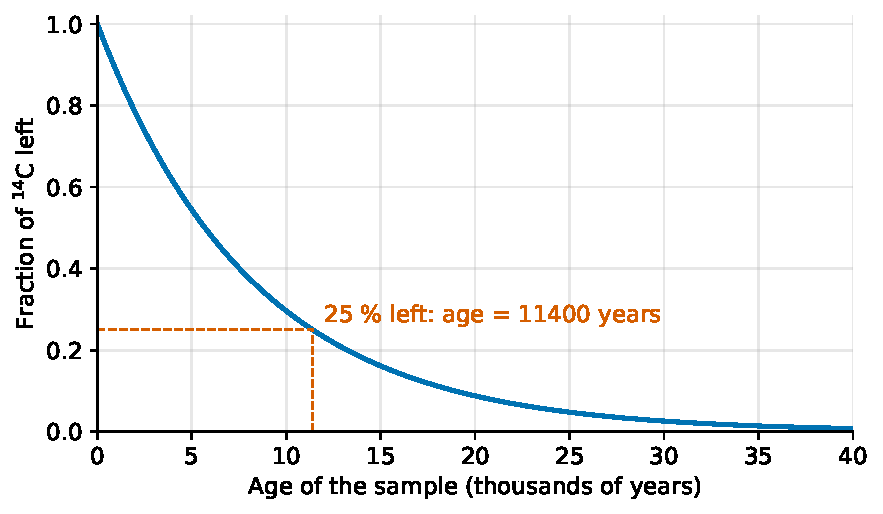
\includegraphics[width=0.7\textwidth]{carbon14}
\caption{Fraction of \iso{14}{C} left in a sample as a function of the time since the death of the organism.}
\label{fig:carbon}
\end{figure}

\begin{examplebox}
\textbf{Dating a bone.} A piece of bone has an activity of $0.058$~Bq per gram of carbon, a quarter of the activity of living matter. Two half-lives have passed, so the animal died $2 \times 5700 = 11\,400$ years ago. In general, from $A = A_0 (1/2)^{t/T_{1/2}}$,
\[
t = T_{1/2}\, \frac{\ln(A_0/A)}{\ln 2}.
\]
The method works for ages up to about 50\,000 years. Beyond that, too little \iso{14}{C} is left to be measured.
\end{examplebox}

Longer-lived nuclides date older objects. The decays of \iso{238}{U} and \iso{235}{U} into lead are used to date rocks, and gave the age of the Earth: 4.5 billion years.

\subsection{Medicine and industry}

\begin{itemize}
  \item \textbf{Medical imaging.} A radioactive tracer is injected and its $\gamma$ rays are detected from outside the body: technetium~99m for bone and heart scans, fluorine~18 attached to glucose for PET scans of tumours.
  \item \textbf{Radiotherapy.} The radiation of cobalt~60 or of particle accelerators is used to destroy tumours; iodine~131, which concentrates in the thyroid, treats thyroid cancers.
  \item \textbf{Industry and everyday life.} Sterilization of medical equipment, measurement of thicknesses, and smoke detectors, in which the $\alpha$ particles of americium~241 ionize the air.
\end{itemize}

\subsection{Radiation and health}

Radiation from radioactive decay is \emph{ionizing}: it can tear electrons from atoms and damage living cells, in particular their DNA. The effect on the body is measured by the \emph{effective dose}, in sieverts (Sv). We are all exposed to natural radiation, from radon, cosmic rays, the rocks and our own potassium~40: on average about $2.4$~mSv per year worldwide~\cite{UNSCEAR2008}. The three basic rules of radiation protection are \emph{time} (stay close to a source for as short a time as possible), \emph{distance} (the intensity decreases as $1/r^2$) and \emph{shielding} (paper for $\alpha$, aluminium for $\beta$, lead or concrete for $\gamma$).

%======================================================================
\section{Nuclear energy: fission and fusion}
%======================================================================

\subsection{Fission}

In 1938, Otto Hahn and Fritz Strassmann found barium among the products of uranium bombarded with neutrons. Lise Meitner and Otto Frisch understood that the uranium nucleus had split in two: this was the discovery of \textbf{fission}. A typical reaction is
\[
\ce{^{235}_{92}U + ^{1}_{0}n -> ^{141}_{56}Ba + ^{92}_{36}Kr + 3 ^{1}_{0}n}, \qquad Q = 173~\text{MeV}.
\]
Many other pairs of fragments are possible. Including the energy released later by the radioactive decays of the fragments, each fission releases about 200~MeV.

The key point is that each fission releases 2 or 3 neutrons (about 2.4 on average), which can cause new fissions: a \textbf{chain reaction}. In a nuclear reactor, the chain reaction is controlled so that, on average, exactly one neutron per fission causes a new fission. This requires:
\begin{itemize}
  \item a \emph{moderator} (water or graphite), which slows down the neutrons, since slow neutrons are much more likely to cause the fission of \iso{235}{U};
  \item \emph{control rods} made of neutron-absorbing materials such as boron or cadmium, which regulate the number of neutrons;
  \item fuel \emph{enriched} in \iso{235}{U}: natural uranium contains only $0.72\%$ of it, and most reactors use 3 to 5\%.
\end{itemize}

\subsection{Fusion}

Fusion joins two light nuclei. The most accessible reaction on Earth is that of deuterium and tritium, two isotopes of hydrogen:
\[
\ce{^{2}_{1}H + ^{3}_{1}H -> ^{4}_{2}He + ^{1}_{0}n}, \qquad Q = 17.6~\text{MeV}.
\]
By momentum conservation, the neutron carries $4/5$ of this energy, 14.1~MeV.

Fusion is difficult because the two nuclei repel each other. To touch, at a distance of about 3~fm, they must overcome an electric potential energy
\[
E_C = \frac{1}{4\pi\varepsilon_0}\frac{e^2}{r} = \frac{1.44~\text{MeV\,fm}}{3.2~\text{fm}} \approx 0.45~\text{MeV}.
\]
Thermal energies are of order $k_B T$, and $k_B T = 0.45$~MeV would require a temperature of 5 billion kelvin. In practice, thanks to quantum tunnelling and to the fastest particles of the thermal distribution, fusion occurs at temperatures of about 150 million kelvin in experimental reactors such as ITER, and 15 million kelvin in the core of the Sun.

\paragraph{The energy of the Sun.} The Sun converts hydrogen into helium through the \emph{proton--proton chain}, whose overall result is
\[
\ce{4 ^{1}H -> ^{4}He + 2 e+ + 2 $\nu_e$}, \qquad Q = 26.7~\text{MeV}.
\]
About $0.7\%$ of the mass of the hydrogen is converted into energy. A small part of it is carried away by the neutrinos, and the rest heats the Sun.

\subsection{Comparing energy sources}

\begin{table}[h]
\centering
\begin{tabular}{lcc}
\toprule
Fuel & Energy per reaction & Energy per kilogram of fuel \\
\midrule
Coal (burning) & about 4 eV & about $3 \times 10^{7}$ J \\
Uranium 235 (fission) & about 200 MeV & $8 \times 10^{13}$ J \\
Deuterium--tritium (fusion) & 17.6 MeV & $3.4 \times 10^{14}$ J \\
\bottomrule
\end{tabular}
\caption{Energy released per kilogram of fuel. For fission, $200~\text{MeV}$ per nucleus of 235~u; for fusion, $17.6~\text{MeV}$ per 5~u of fuel.}
\label{tab:energy}
\end{table}

One kilogram of uranium~235 releases as much energy as about 3000 tonnes of coal (Table~\ref{tab:energy}). This is the ratio of nuclear to chemical energies: MeV against eV.

%======================================================================
\section{Simulating with Python}
%======================================================================

The programs that come with these notes are in the repository
\begin{center}\url{https://github.com/daoudizakaria/Radioactive_Decay}\end{center}
They require Python~3 with the \texttt{numpy}, \texttt{pandas} and \texttt{matplotlib} libraries (\texttt{pip install -r requirements.txt}).

\begin{description}[leftmargin=1em]
  \item[\texttt{radioactivity.py}] The simplest program. It solves the decay law with Euler's method for a nuclide of your choice and compares it with the exact solution.
  \item[\texttt{nuclear.py}] The complete program, with four simulations: (1) decay of a nuclide and its activity, (2) a parent--daughter chain, (3) a chain with branching, (4) Monte Carlo decay. The results can be exported to a CSV file, for example to be analysed in a spreadsheet.
  \item[\texttt{nuclear\_energy.py}] Binding energies, the liquid drop model and $Q$-values, computed from the AME2020 masses.
  \item[\texttt{make\_figures.py}] Produces all the figures of these notes.
\end{description}

\noindent The half-lives are in \texttt{nuclides\_data.py} and \texttt{nuclides.csv}; the masses and decay modes of all known nuclides are in the folder \texttt{data}. The tests in \texttt{tests/} check the code against exact results (\texttt{python3 -m unittest discover tests}).

%======================================================================
\section{Exercises}
%======================================================================

Exercises marked $\star$ use the \emph{Going further} material. Answers are given at the end.

\begin{enumerate}[label=\textbf{\arabic*.}]
  \item \textbf{Composition.} Give the number of protons, neutrons and nucleons of \iso{14}{C}, \iso{56}{Fe}, \iso{131}{I} and \iso{235}{U}.

  \item \textbf{Size of nuclei.} Using Eq.~\eqref{eq:radius}, compute the radii of \iso{4}{He}, \iso{56}{Fe} and \iso{238}{U}. How many times larger in volume is \iso{238}{U} than \iso{4}{He}?

  \item \textbf{Binding energy of the deuteron.} The atomic mass of deuterium \iso{2}{H} is $2.014102$~u. Using the masses of the hydrogen atom ($1.007825$~u) and of the neutron ($1.008665$~u), compute the binding energy of the deuteron and its binding energy per nucleon. Compare with \iso{4}{He}.

  \item \textbf{Decay equations.} Identify the nucleus X in the following decays and name their type:
  (a) \ce{^{226}_{88}Ra -> $\mathrm{X}$ + ^{4}_{2}He};
  (b) \ce{^{131}_{53}I -> $\mathrm{X}$ + e- + $\bar{\nu}_e$};
  (c) \ce{^{18}_{9}F -> $\mathrm{X}$ + e+ + $\nu_e$};
  (d) $\nuc{60}{28}{Ni}^* \to \mathrm{X} + \gamma$.

  \item \textbf{Iodine 131.} After the Chernobyl and Fukushima accidents, iodine~131 ($T_{1/2} = 8.02$ days) was a major concern during the first weeks. What fraction of it is left after 24 days? After 80 days?

  \item \textbf{Activity of a source.} A cobalt~60 source used in radiotherapy has an activity of $\SI{2e14}{Bq}$. What is its activity after 10 years? Its half-life is 5.27 years. How many \iso{60}{Co} atoms does it contain initially?

  \item \textbf{Radiocarbon.} A piece of wood from an archaeological site has an activity of $0.16$~Bq per gram of carbon, while living wood has $0.23$~Bq/g. How old is it?

  \item \textbf{Chain of decays.} How many $\alpha$ and $\beta^-$ decays transform \iso{232}{Th} into stable \iso{208}{Pb}?

  \item \textbf{Energy of the Sun.} The Sun radiates $\SI{3.8e26}{W}$. Using the $Q$-value of the proton--proton chain, estimate how many helium nuclei it produces per second, and the mass of hydrogen it consumes per second.

  \item \textbf{A natural nuclear reactor.} Today, natural uranium contains $0.7204\%$ of \iso{235}{U} and $99.2742\%$ of \iso{238}{U}. Because \iso{235}{U} decays faster, it was more abundant in the past. Compute the proportion of \iso{235}{U} two billion years ago. (About 1.7 to 2 billion years ago, natural chain reactions took place in the uranium deposit of Oklo, in Gabon.)

  \item[$\star$\textbf{11.}] \textbf{Mean life.} Show that the mean lifetime of a nucleus is $\tau = 1/\lambda$ and that, after a time $\tau$, a fraction $1/e \approx 37\%$ of the nuclei remain.

  \item[$\star$\textbf{12.}] \textbf{Most stable isobar.} Using the liquid drop formula with the coefficients of Section~\ref{sec:liquid}, find the most stable value of $Z$ for $A = 56$ and for $A = 208$. Compare with iron and lead.

  \item[$\star$\textbf{13.}] \textbf{Maximum of the daughter.} In the chain P $\to$ D, show from Eq.~\eqref{eq:bateman} that the number of daughter nuclei is maximum at
  \[
  t_{\max} = \frac{\ln(\lambda_D/\lambda_P)}{\lambda_D - \lambda_P}
  \]
  and compute it for \iso{140}{Ba} $\to$ \iso{140}{La}. Show that at this time the activities of parent and daughter are equal.

  \item[$\star$\textbf{14.}] \textbf{Stability of Euler's method.} Show that Euler's method gives $N_i = N_0 (1 - \lambda \Delta t)^i$. For which values of $\lambda \Delta t$ does $N_i$ decrease without changing sign? Check your answer with \texttt{radioactivity.py}.
\end{enumerate}

\subsection*{Answers}

\begin{enumerate}[label=\textbf{\arabic*.}]
  \item \iso{14}{C}: 6, 8, 14. \iso{56}{Fe}: 26, 30, 56. \iso{131}{I}: 53, 78, 131. \iso{235}{U}: 92, 143, 235.
  \item $1.9$~fm, $4.6$~fm and $7.4$~fm. The volume ratio is $238/4 \approx 60$.
  \item $\Delta m = 0.002388$~u, $B = 2.22$~MeV, $B/A = 1.11$~MeV, more than six times less than \iso{4}{He} (7.07~MeV): the deuteron is very weakly bound.
  \item (a) \iso{222}{Rn}, $\alpha$ decay. (b) \iso{131}{Xe}, $\beta^-$ decay. (c) \iso{18}{O}, $\beta^+$ decay. (d) \iso{60}{Ni}, $\gamma$ emission.
  \item 24 days is 3 half-lives: $1/8 = 12.5\%$. After 80 days (about 10 half-lives), $(1/2)^{80/8.02} \approx 0.1\%$.
  \item $A = \SI{2e14}{Bq} \times (1/2)^{10/5.27} = \SI{5.4e13}{Bq}$. $N = A/\lambda = \SI{2e14}{Bq} \times \SI{1.66e8}{s}/0.693 = \num{4.8e22}$ atoms, about 4.8~g of cobalt~60.
  \item $t = 5700 \times \ln(0.23/0.16)/\ln 2 \approx 3000$~years.
  \item $232 - 208 = 24 = 6 \times 4$: 6 $\alpha$ decays, which lower $Z$ from 90 to 78; 4 $\beta^-$ decays bring it to 82.
  \item Each chain releases $26.7~\text{MeV} = \SI{4.28e-12}{J}$, so $\SI{3.8e26}{W}/\SI{4.28e-12}{J} = \num{8.9e37}$ helium nuclei per second. They consume $4 \times \num{8.9e37} \times \SI{1.67e-27}{kg} \approx \SI{6e11}{kg}$ of hydrogen per second, 600 million tonnes.
  \item With $\lambda_{235} = \ln 2 / 7.04\times10^8~\text{y}$ and $\lambda_{238} = \ln 2 / 4.463\times10^9~\text{y}$, the ratio \iso{235}{U}/\iso{238}{U} was $0.007257 \times e^{(\lambda_{235}-\lambda_{238}) \times 2\times10^9~\text{y}} = 0.0381$, that is $3.7\%$ of \iso{235}{U}, comparable to the fuel of modern reactors.
  \item The integral is computed by parts. $N(\tau)/N_0 = e^{-1}$.
  \item $Z = 56/(2 + 0.0154 \times 56^{2/3}) = 25.2$, close to iron ($Z = 26$). $Z = 208/(2 + 0.0154 \times 208^{2/3}) = 81.8$, close to lead ($Z = 82$).
  \item Set $dN_D/dt = 0$. For \iso{140}{Ba} $\to$ \iso{140}{La}, $t_{\max} = 5.7$~days. At $t_{\max}$, $dN_D/dt = \lambda_P N_P - \lambda_D N_D = 0$, so $A_P = A_D$ (see Figure~\ref{fig:chains}b).
  \item $N_i$ decreases without changing sign when $0 < \lambda \Delta t < 1$; it oscillates for $1 < \lambda\Delta t < 2$ and blows up for $\lambda\Delta t > 2$.
\end{enumerate}

%======================================================================
\begin{thebibliography}{9}

\bibitem{NUBASE2020}
F.~G.~Kondev, M.~Wang, W.~J.~Huang, S.~Naimi, and G.~Audi,
``The NUBASE2020 evaluation of nuclear physics properties,''
\emph{Chinese Physics C} \textbf{45}, 030001 (2021).

\bibitem{AME2020}
M.~Wang, W.~J.~Huang, F.~G.~Kondev, G.~Audi, and S.~Naimi,
``The AME 2020 atomic mass evaluation (II). Tables, graphs and references,''
\emph{Chinese Physics C} \textbf{45}, 030003 (2021).

\bibitem{CODATA2018}
E.~Tiesinga, P.~J.~Mohr, D.~B.~Newell, and B.~N.~Taylor,
``CODATA recommended values of the fundamental physical constants: 2018,''
\emph{Reviews of Modern Physics} \textbf{93}, 025010 (2021).

\bibitem{Bateman1910}
H.~Bateman,
``Solution of a system of differential equations occurring in the theory of radioactive transformations,''
\emph{Proceedings of the Cambridge Philosophical Society} \textbf{15}, 423 (1910).

\bibitem{UNSCEAR2008}
UNSCEAR,
\emph{Sources and Effects of Ionizing Radiation}, UNSCEAR 2008 Report to the General Assembly, Volume I, United Nations (2010).

\bibitem{Krane}
K.~S.~Krane,
\emph{Introductory Nuclear Physics}, Wiley (1988).

\bibitem{Basdevant}
J.-L.~Basdevant, J.~Rich, and M.~Spiro,
\emph{Fundamentals in Nuclear Physics: From Nuclear Structure to Cosmology}, Springer (2005).

\bibitem{MartinShaw}
B.~R.~Martin and G.~Shaw,
\emph{Nuclear and Particle Physics: An Introduction}, 3rd ed., Wiley (2019).

\end{thebibliography}

\noindent For further reading, Krane~\cite{Krane} is a classic undergraduate textbook; Basdevant, Rich and Spiro~\cite{Basdevant} and Martin and Shaw~\cite{MartinShaw} are more modern introductions.

\end{document}
